\documentclass[11pt, oneside]{article}       
\usepackage{geometry}                        
\geometry{letterpaper}                           
\usepackage{graphicx}                        
\usepackage{float}
\usepackage{amssymb}

\usepackage{fancyhdr}
\usepackage{fancyhdr}
\fancyhead[L]{October 6, 2017}
\fancyhead[C]{SE 3XA3 Test Plan}
\fancyhead[R]{$\int_{}^{}$n2gr8}
\pagestyle{fancy}


%SetFonts

%SetFonts


\title{Requirements Document}
\author{Anthony Guirguis (guirguia) \\ Hoda Mohammadi (mohamh8) \\ Mikolaj Hrycko (hryckom)}

\date{October 6, 2015}

\begin{document}
\maketitle
\newpage
\tableofcontents
\newpage

\listoftables
\listoffigures

\newpage
\section*{Revision History}

\begin{table}[hp]
\caption{Revision History: Requirements Document}
\begin{center}
\label{tab:}
\begin{tabular}{|c|c|c|c|}
\hline
\textbf{DATE} & \textbf{DEVELOPER} & \textbf{CHANGE} & \textbf{REVISION}\\
\hline
October 6, 2015 & Anthony Guirguis & Initial Draft & 0\\
\hline
October 6, 2015 & Hoda Mohammadi & Initial Draft & 0\\
\hline
October 6, 2015 & Mikolaj Hrycko & Initial Draft & 0\\
\hline
\end{tabular}
\end{center}
\label{default}
\end{table}

\newpage
\section{Project Drivers}
\subsection{The Purpose of the Project}
\subsubsection{The User Business or Background of the Project Effort}
This project is a  reimplementation of a JavaScript math library called MathJS and we intend on going a step further than the original implementation and creating a website that uses our implementation. We plan on allowing users to input derivative, integral and numerical expression problems that can be solved and outputted straight to the user. The original library featured a flexible expression parser with support for symbolic computation and a large set of built-in functions. Our motivation to make this project is to make a place where complex mathematical expressions can be solved with little effort from the user and to offer a user-friendly service instead of just developing an API like MathJS.

\subsubsection{Goals of the Project}
Our product will allow users to input a variety of mathematical expressions and obtain the answers to these expressions on an elegant, easy to use website. The goals for this project are creating a JavaScript program that implements a library similar to MathJS, documenting the processes involved in making the project and getting a website to host the program. The website is there so users can easily access the program and use it.


\subsection{The Stakeholders}
\subsubsection{The Client}
An external entity that will be reviewing the project and is interested in implementing a math expression solver for general as well as specific use.

\subsubsection{The Customer}
The customer of our project is the general public, and more specifically students, teachers and people working with math expressions daily.

\subsubsection{Other Stakeholders}
\begin{itemize}
\item Members of the public
\subitem Represents the rest of the user base. No extra knowledge or involvement required, due to the easy to use nature of the website.
\end{itemize}


\subsubsection{The Hands-On-Users of the Product}
\begin{itemize}
\item University Students
\subitem Interacts with website
\subitem Master at navigating the web
\subitem Ability to access completed website
\end{itemize}


\subsubsection{Personas}
\begin{itemize}
\item Name: Joe Schmo
\subitem Age: 20
\subitem Job: Unemployed
\subitem Family: Jake Cane, Father
\subitem Hobbies: Researching the psychological effects of sleep deprivation
\subitem City: Llanfairpwllgwyngyllgogerychwyrndrobwllllantysiliogogogoch, United Kingdom
\subitem Favourite Food: Fermented cucumbers
\subitem Favourite Music: Classic Pop
\subitem Likes: Math, Integrals, Computers
\subitem Dislikes: Short city names, sleeping
\subitem Attitude to Technology: Positive
\subitem Attitude to Money: Indifferent
\end{itemize}


\subsubsection{Priorities Assigned to Users}

\textbf{Key Users:}\\
The Customer\\
\\
\textbf{Secondary Users:}\\
The General Public\\
\\
\textbf{Unimportant Users:}\\
The General Public\\


\subsubsection{User Participation}
\textbf{The Customer}\\
No input necessary.\\
\\
\textbf{The General Public:}\\
No input necessary.\\


\subsubsection{Maintenance Users and Service Technicians}
\textbf{Project Maintenance Team}\\
These users will maintain and update the code in the project and the performance of the website.


\newpage
%---------------------------------------------------------------------
\section{Project Constraints}
\subsection{Mandated Constraints}
\subsubsection{Solution Constraints}
Description: The product shall operate on computer browsers that allow JavaScript to run through a website hosting server.
\\
\\
Rationale: The user will be using a desktop/laptop and browser that is not outdated to access our site.
\\
\\
Fit criterion: Our website will be usable to users with browsers that have an updated version of JavaScript.
\\
\\
\\
Description: The program shall be used only when connected to the internet so that user inputs can be processed.
\\
\\
Rationale: The internet connection of the user should be appropriate for the program to run.
\\
\\
Fit criterion: The user shall have an internet connection with at least 100kbs upload and download speed
\\
\\
\\
Description: The product shall resize to the different resolutions of internet browsers and the different sizes that browsers use.
\\
\\
Rationale: The user should be able to resize the browser with the program resizing accordingly.
\\
\\
Fit criterion: The program shall be able to resize on browsers on desktops and laptops. The minimum size allowed is 720 by 1080 pixels and the maximum is 7680 by 4320 pixels.

\subsubsection{Implementation Environment of the Current System}
\subsubsection*{Implementation Environment of the Current System}
\begin{figure}[H] %  figure placement: here, top, bottom, or page
   \centering
   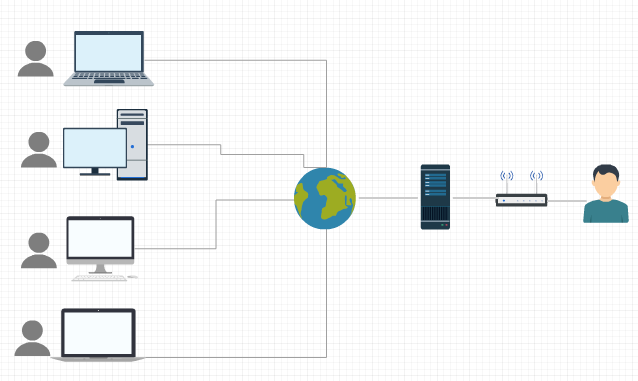
\includegraphics[width=6in]{DeploymentDiagram.png}
   \caption{Implementation Environment}
   \label{fig:example}
\end{figure}

\subsubsection{Partner or Collaborative Applications}
The program relies on React, a JavaScript library to properly layout the user interface to the website. It also relies on a browser supporting JavaScript and a web-hosting server.


\subsubsection{Off-the-Shelf Software}
For the product to be executed the following off-the-shelf software is required:\begin{itemize}
\item
A web browser
\item
JavaScript (Available from https://java.com/en/download/)
\item
A client where the web browser can run (i.e. desktop, laptop)
\end{itemize}

All three of the OTS software can be received for free off the Internet.


\subsubsection{Anticipated Workspace Environment}
The anticipated workplace environment for the product is anywhere. As long as some sort of internet connection is present, the website can be accessed.


\subsubsection{Schedule Constraints}
There is no schedule constraint that affects the product requirements. However, a deadline of the beginning of December has been given to finish the project.


\subsubsection{Budget Constraints}
There are no budget constraints as everything that is required is either open source or free to use.


\subsubsection{Enterprise Constraints}
The program will be free to use and available on desktop and laptop platforms, that have browsers capable of running JavaScript.


\subsection{Naming Conventions and Terminology}
\subsubsection{Definitions of All Terms, Including Acronyms, Used by Stakeholders Involved in the Project}

\begin{table}[H]
\caption{Definitions}
\begin{center}
\begin{tabular}{|c|c|}
\hline
\hline
ACRONYM/ABBREVIATION & INTENDED MEANING\\
\hline
JS & JavaScript\\
\hline
HTML &Hypertext Markup Language, used mainly in website creation\\
\hline
OS & Operating System\\
\hline
React & a JavaScript library for building user interfaces\\
\hline
\end{tabular}
\end{center}
\label{default}
\end{table}%



\subsection{Relevant Facts and Assumptions}
\subsubsection{Relevant Facts}
Some relevant facts for this project are that there are 60,000 lines of code in the library. The library has a Apache license and JavaScript is needed to start using the library.

\subsubsection{Business Rules}
The documentation will be equally written by all members of the group. Members will specifically code parts of the project that they feel are stronger at coding.

\subsubsection{Assumptions}
Some assumptions about the project are the web-hosting server will be free. Also, React will be available for us to use to build the user interface for the website. In terms of coding, the parser will be coded first, as the rest of the code is reliant on this.


\newpage
%---------------------------------------------------------------------
\section{Functional Requirements}
\subsection{The Scope of the Work}
\subsubsection{The Current Situation}
\begin{figure}[H] %  figure placement: here, top, bottom, or page
   \centering
   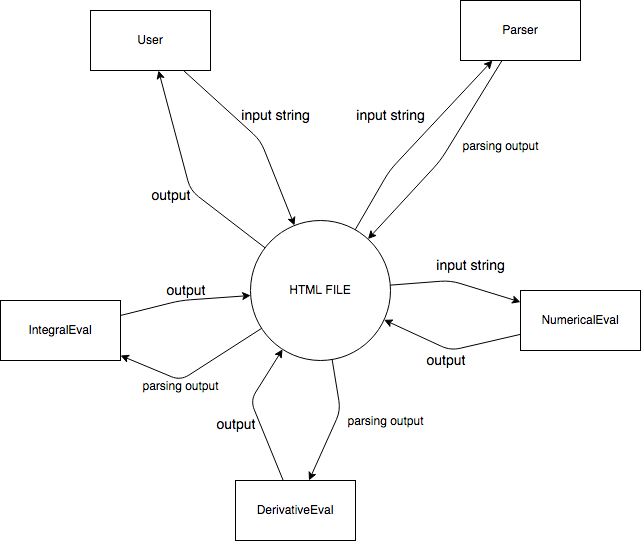
\includegraphics[width=6in]{DataFlowDiagram.png}
   \caption{Data Flow Diagram}
   \label{fig:example}
\end{figure}


\subsubsection{The Context of the Work}
\begin{figure}[H] %  figure placement: here, top, bottom, or page
   \centering
   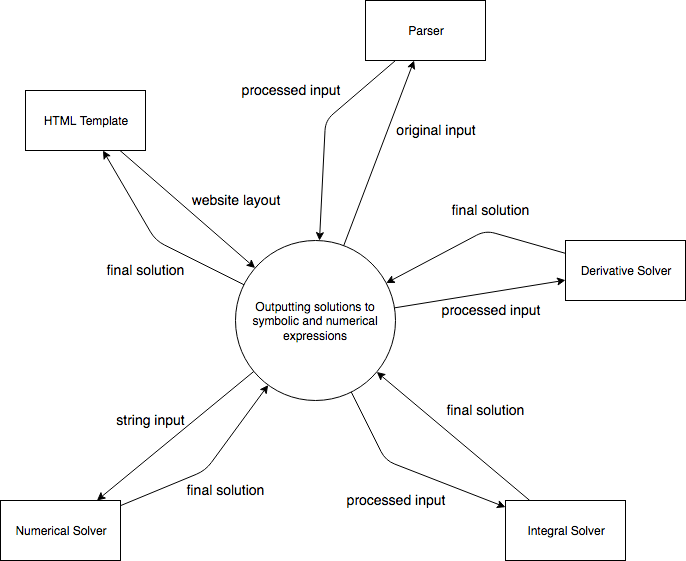
\includegraphics[width=6in]{WorkContextDiagram.png}
   \caption{Work Context Diagram}
   \label{fig:example}
\end{figure}


\subsubsection{Work Partitioning}
\begin{table}[H]
\caption{Work Partitioning Part I}
\begin{center}
\begin{tabular}{|c|c|c|c|}
\hline
Event Number & Event Name & Input & Output\\
\hline
1 & Parser manipulates input & Website input label & Developer code\\
\hline    
2 & Parser organizes data  & Developer code & Developer code\\
\hline    
3 & Functions process parser data & Developer code & Developer code\\
\hline
4 & Data to Site & Developer code & Website\\
\hline    
5 & Website creation & Developer code & Website\\
\hline    
6 & Final Edits & Developer code & Website\\
\hline
\end{tabular}
\end{center}
\label{default}
\end{table}%
 
\begin{table}[H]
\caption{Work Partitioning Part II}
\begin{center}
\begin{tabular}{|c|c|}

\hline
Event Number & Summary of BUC\\
\hline
1 & Parser receives input from user via website which will be later created \\
\hline
2 & Parsed data will be organized in a\\ &way to make it easy to manipulate the data\\
\hline
3 & Create functions that process the data \\
\hline
4 & Sends processed data from code to the\\ &front end of a website that is later created\\
\hline
5 & Create an easy to use website that will allow the\\ &user to input a mathematical problem and receive\\ &a solution for their given problem on the website\\
\hline
6 & Finishing edits to the project\\
\hline

\end{tabular}
\end{center}
\label{default}
\end{table}%



\subsubsection{Specifying a Business Use Case (BUC)}
Not applicable.


\subsection{Business Data Model \& Data Dictionary}
\subsubsection{Business Data Model}
\begin{figure}[H] %  figure placement: here, top, bottom, or page
   \centering
   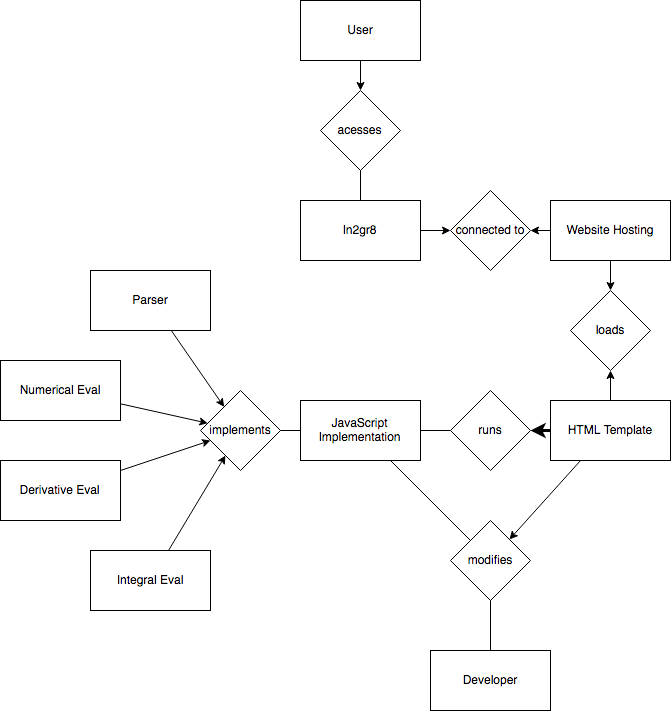
\includegraphics[width=6in]{BusinessDataModel.png}
   \caption{Business Data Model}
   \label{fig:example}
\end{figure}

\subsubsection{Data Dictionary}
\begin{table}[H]
\caption{Data Dictionary}
\begin{center}
\begin{tabular}{|c|c|c|}
\hline
Name & Content &Type\\
\hline    
Developer & Developer Name & Class\\
\hline    
User & Username & Class\\
\hline    
In2gr8 & In2gr8 Instance & Class\\
\hline
Website Hosting & IP + Domain & Class\\
\hline    
HTML Template & Template Name & class\\
\hline
JavaScript Implementation & JS Function & Class\\
\hline    
Parser & Parser Input & Class\\
\hline    
Numerical Eval & Parser output + Final output & Class\\
\hline    
Derivative Eval & Parser output + Final output & Class\\
\hline    
Integral Eval & Parser output + Final output & Class\\
\hline    



Developer Name & String & Attribute/ Element\\
\hline
Username & String & Attribute/ Element\\
\hline
In2gr8 Instance & Created Instance ID & Attribute/ Element\\
\hline
IP & IP address & Attribute/ Element\\
\hline
Domain & Domain address & Attribute/ Element\\
\hline
Template Name & String & Attribute/ Element\\
\hline
JS Function & Document Description String & Attribute/ Element\\
\hline
Parser Input & String & Attribute/ Element\\
\hline
Parser output & Array & Attribute/ Element\\
\hline
Final output & String & Attribute/ Element\\
\hline
\end{tabular}
\end{center}
\label{default}
\end{table}%


\subsection{The Scope of the Product}
\subsubsection{Project Boundary}



\subsubsection{Product Use Case Table}



\subsubsection{Individual Product Use Cases}



\subsection{Functional Requirements}
\begin{itemize}
\item
Upon accessing the final website with the given domain, a new browser window will appear.
\subitem
Fit Criterion or Test Case: \\
Does a new instance of the website appear upon accessing the website?

\item
The website can be accessed from any of the popular internet browsers such as Chrome, Firefox, Opera, and Microsoft Edge.
\subitem
Fit Criterion or Test Case: \\
Attempt to access the website from different internet browsers.

\item
The website will remain idle and nothing will happen until a user passes through an input
\subitem
Fit Criterion or Test Case: \\
Access the website and don’t submit any input to see if the website performs any actions without any user input.

\item
Upon receiving input, the website will begin to solve for a solution to the given problem.
\subitem
Fit Criterion or Test Case: \\
Provide user input to see if the website begins to solve the given problem.

\item
Upon accessing the website, the input and output fields will remain empty which is their default state.
\subitem
Fit Criterion or Test Case: \\
Access the website before submitting user input to ensure that a new instance is created every time the website is accessed.

\item
Upon a solution being found, the solution will be displayed to the user and allow the user to input a new mathematical problem to be solved.
\subitem
Fit Criterion or Test Case: \\
Return the solution to the given problem and have the ability to enter a new problem to be solved..

\item
If there is any errors with the user input such as unrecognized characters or improper format, the website will return an error indicating that the user’s input was incorrect. There will be no attempt to solve the mathematical problem is the input is incorrect.

\subitem
Fit Criterion or Test Case: \\
Test improper formats or unrecognized characters to ensure that the program returns an error and does not continue until the input is fixed.

\end{itemize}

\newpage
%---------------------------------------------------------------------
\section{Non-functional Requirements}
\subsection{Look and Feel Requirements}
\subsubsection{Appearance Requirements}
The product shall have one neutral theme color to not distract users from the function of the website. In2gr8 shall have labels for the input boxes to indicate the type of input that is required. The In2gr8 shall also have the name of the product visible on all pages of the website. It shall have a clear division of sections for each function that it does.




\subsubsection{Style Requirements}
The product shall provide a professional atmosphere that is appropriate for educational and workplace use. It should seem trustworthy so the users feel the results they receive are accurate.




\subsection{Usability and Humanity Requirements}
\subsubsection{Ease of Use Requirements}
The product shall provide all the steps taken to solve the problem to make the user feel confident the results are accurate. It shall make it easy for the user to make changes to their initial input and make it easy to clear all inputs and start over. The product shall be used by people with very little knowledge of the math concepts, the english language or training in the use of the product. The product shall be usable by users of ages 8 and up.


\subsubsection{Personalization and Internationalization Requirements}
The product shall allow the users to pick their preferred units for certain inputs/outputs and pick the function that they would like to use.

\subsubsection{Learning Requirements}
A person with access to internet and basic knowledge of browsing internet shall learn to use the product in very little to no time.


\subsubsection{Understandability and Politeness Requirements}
The product shall use universal math symbols.


\subsubsection{Accessibility Requirements}
The product shall conform to the ontarians with disabilities act policies that are related to the product.


\subsection{Performance Requirements}
\subsubsection{Speed and Latency Requirements}
The product shall compute simple solutions within 2 seconds and more complicated ones within 5 seconds. The page loading shall have a maximum response time of 2 seconds.


\subsubsection{Safety-Critical Requirements}
The website shall not access/compromise the user’s machine or data.


\subsubsection{Precision or Accuracy Requirements}
The product shall return solutions with 4 decimal accuracy and in exact form when possible. The product shall avoid rounding outputs as much as possible to avoid inaccuracy. The percentage error for the results shall be +/- 0.5%.


\subsubsection{Reliability and Availability Requirements}
The product shall be available for use 24 hours per day, 365 days per year.


\subsubsection{Robustness or Fault-Tolerance Requirements}
The other functions of the program shall continue to operate should one function fail or if it is down for maintenance.


\subsubsection{Capacity Requirements}
The website shall not exceed the server load.


\subsubsection{Scalability or Extensibility Requirements}
The server shall handle a load of approximately 10 users per day within the next year.  


\subsubsection{Longevity Requirements}
The product shall be expected to operate until the end of course term and continue to operate for at least one year, as long as maintenance and update is performed when needed.


\subsection{Operational and Environmental Requirements}
\subsubsection{Expected Physical Environment}
The product shall be used in quiet study areas or classrooms or anywhere that there is a device with access to the internet.


\subsubsection{Requirements for Interfacing with Adjacent Systems}
The products shall work on the latest releases of Chrome, Safari and FireFox and it shall be accessible from computer, tablet and mobile phones.


\subsubsection{Productization Requirements}
The product shall be hosted on a website to become distributable.

\subsubsection{Release Requirements}
The product shall be updated to fix any bugs after one month of release and from then on a maintenance release will be offered to users once a year.


\subsection{Maintainability and Support Requirements}
\subsubsection{Maintenance Requirements}
The product shall be updated overnight when maintenance is being performed.


\subsubsection{Supportability Requirements}
The product shall have a user manual page to demonstrate how the product can be used and a help section for users to ask any questions they might have.


\subsubsection{Adaptability Requirements}
The product shall run on any device that has a web browser.


\subsection{Security Requirements}
\subsubsection{Access Requirements}
Anyone shall access the website to use all features but only team members shall have access to the help requests made by users.


\subsubsection{Integrity Requirements}
The product shall not change or delete any of the software code or alter the input user data.


\subsubsection{Privacy Requirements}
The product shall not collect any user data other than the information they input into the system which shall be deleted from the system once the user exists the application.


\subsubsection{Audit Requirements}
N/A


\subsubsection{Immunity Requirements}
N/A


\subsection{Cultural Requirements}
This product shall be able to compute solutions for various units such as metric and imperial systems. It shall also minimize the use of words and use symbols instead to accommodate users with different languages.


\subsection{Legal Requirements}
\subsubsection{Compliance Requirements}
This website shall not compromise any laws.


\subsubsection{Standards Requirements}
This website shall adhere to the MIT Open License.


\newpage
%---------------------------------------------------------------------
\section{Project Issues}
\subsection{Open Issues}
N/A


\subsection{Off-the-shelf Solutions}
\subsubsection{Ready-Made Products}
\begin{itemize}
\item Servers
\end{itemize}


\subsubsection{Reusable Components}
N/A


\subsubsection{Products That Can Be Copied}
Since this is based off an open-sourced project, the original implementation can be useful for guidance with the base code for this new open source project.


\subsection{New Problems}
\subsubsection{Effects on the Current Environment}
This new service we’re offering will be a new addition to the already massive pool of websites that already exist. Therefore this new website will not have much if any affect on the environment. The only issue that may arise is if there is too much traffic to the website, where we would end up having to upgrade our servers.
\subsubsection{Effects on the Installed Systems}
There will be no effect on already existing system as the new system will be a new instance of the service.

\subsubsection{Potential User Problems}
N/A

\subsubsection{Limitations in the Anticipated Implementation Environment That May Inhibit the New Product}
The only limitation that may be experienced is if the traffic is extremely high on our website, which will result in us having to upgrade our server.

\subsubsection{Follow-Up Problems}
Some problems that may be experienced include not being able to develop a well made and easy to use website since our main priority is getting all our functions to function properly. We are limited by time but we hope to be able to have a fully functional website that’s user friendly and has some nice aesthetics by the end of the semester.


\subsection{Tasks}
\subsubsection{Project Planning}
\begin{table}[H]
\caption{default}
\begin{center}
\begin{tabular}{|c|c|c|}
\hline
Task    & Completer?s Role & Timeline\\
\hline
Parsing Implementation & Software Engineers & Oct 12th\\
\hline
JavaScript design/functions & Software Engineers & Oct 30th\\
\hline
HTML implementation & Software Engineers & Nov 5rd\\
\hline
Hosting & Software Engineers & Nov 25rd\\
\hline
Maintenance & Software Engineers & Yearly\\
\hline
\end{tabular}
\end{center}
\label{default}
\end{table}%


\subsubsection{Planning of the Development Phases}
Phase 1 Parsing Implementation:
This phase is what the rest of the project depends on as we must be able to parse the user's’ input and organize the data in a way to make it easier to manipulate all the data. Organizing all the data to be as specific as possible will make it easier for us to develop the functions since the user’s input will be split up and easily accessible.

Phase 2 Different Mathematical Functions Implementations:
In this phase, we will create all the different functions for each type of mathematical problems. A few examples include finding the derivative, finding the zeros, etc. As the semester goes by, the more excess time we have, the more mathematical problems we will support.

Phase 3 Website development and Hosting Implementation:
After the addition of support for different mathematical problems, a website will be created in order to offer a user-friendly experience where users can input their mathematical problem and receive a nicely formatted solution.


\subsection{Migration to the New Product}
\subsubsection{Requirements for Migration to the New Product}
N/A.


\subsubsection{Data That Has to Be Modified or Translated for the New System}
N/A.


\subsection{Risks}
N/A.


\subsection{Costs}
None since one of the group members already has a server in place and the domain used will be a free domain offered by the hosting company.

\subsection{User Documentation and Training}
\subsubsection{User Documentation Requirements}
N/A.


\subsubsection{Training Requirements}
N/A.


\subsection{Waiting Room}
N/A.


\subsection{Ideas for Solutions}
An efficient way to parse a user’s input could be to use the split function in order to split the user’s input around every space, that way you can have each term of a function in a separate index in an array. Then you can search through the array and search for brackets in order to group up everything in between brackets, if applicable. To do all of this however, would require the assumption that a user has a space between each term.
\end{document}  






